\chapter{Computer Networks}

\section{Introduction}

As humanity has grown and dispersed across the globe over time, the need for faster and more reliable ways to connect people has become paramount.

With the revolutionary invention of the computer, this connection has become easier, faster, and more reliable than ever before. Over time, communication has evolved beyond human interaction to include machine-to-machine communication, as seen in Internet of Things (IoT) applications and many other technologies.

This chapter explores how devices and computers communicate with each other, examining connection methods, protocols, and real-world applications.

\section{Computer Network}
a collection of computers , other devices , and/or
peripherals connected together through connecting
media (Ethernet cables and/or WIFI) to perform certain task that needs a cooperation between two or more devices such as:
\begin{itemize}
	\item File Sharing
	\item Devices Sharing
	\item Software Sharing with multi-user licenses.
	\item Voice and Video calls
	\item video streaming
	\item CCTV 
	\item Share Internet Access
\end{itemize}

\section{Network Elements}
Any computer network consists of two main parts: 
\begin{enumerate}
	\item \textbf{Hardware}
	\begin{itemize}
		\item Devices : Computers - Printers - Phone - Routers - Switches
		\item Mediums : Wired - Wireless - Satellites
		
	\end{itemize}
	
	
	
	\item \textbf{Software}
	\begin{itemize}
		\item Messages : Information that travels over the medium such as Mails-WhatsApp….etc
		\item Protocols : Governs how messages flow across network such as http –https-FTP-RDP
	\end{itemize}
\end{enumerate}

\begin{figure}[!h]
	\centering
	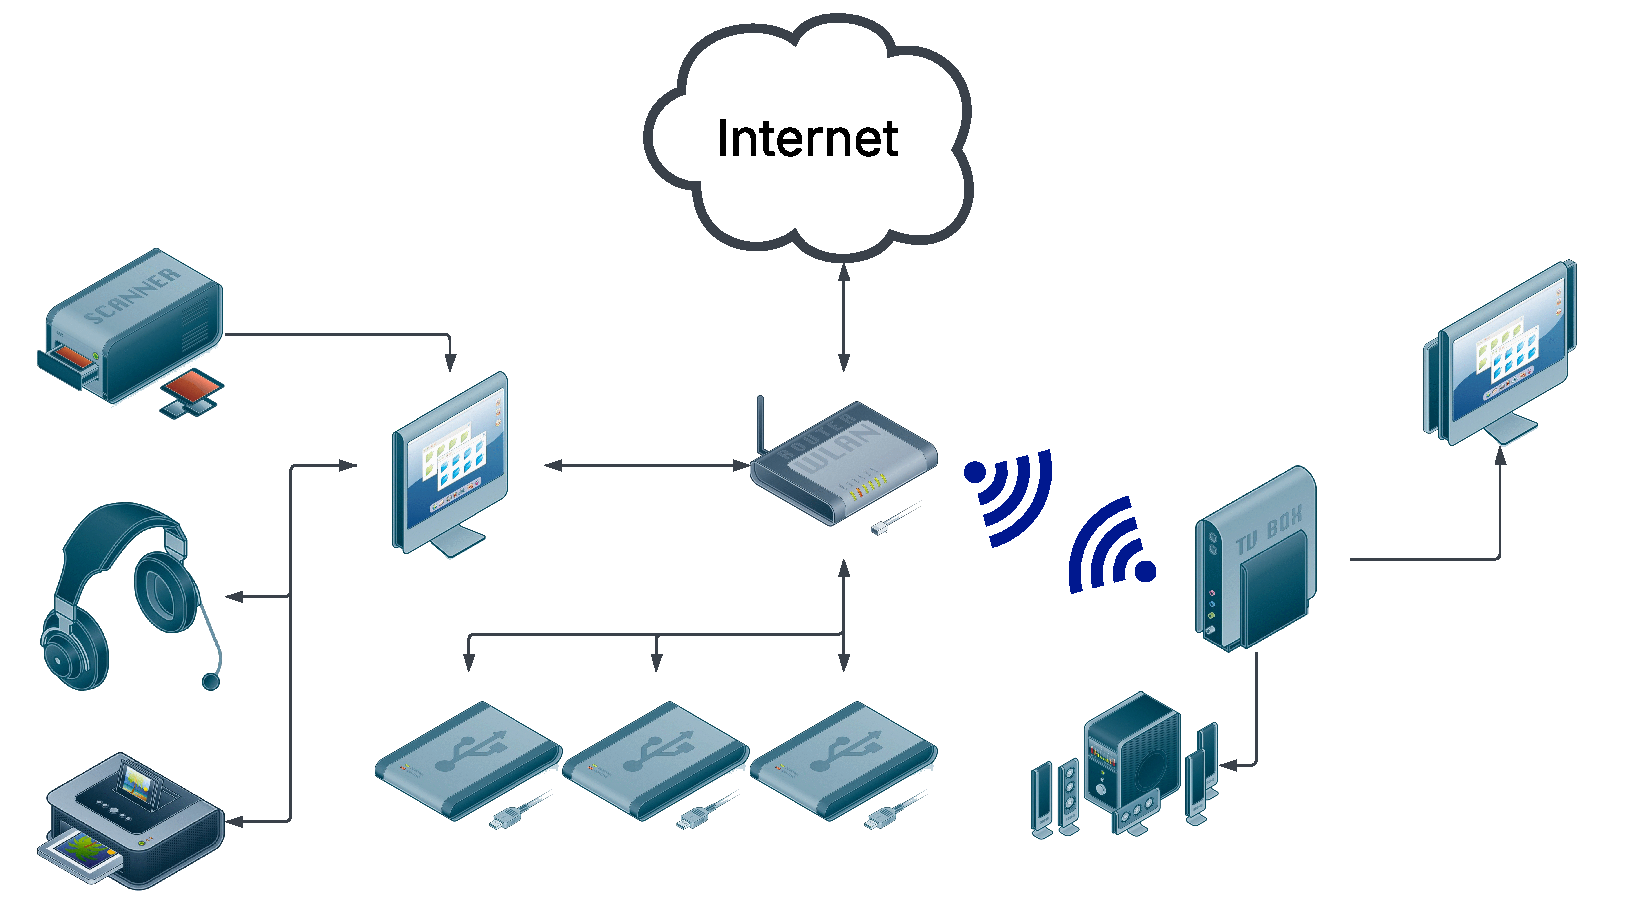
\includegraphics[width=0.7\linewidth]{figures/network1}
	\caption{Example of a network}
	\label{fig:network1}
\end{figure}


\section{Network Basic Terminologies}



\noindent

\begin{minipage}[c]{0.6\textwidth}
	\subsection{Hub}
	A basic physical device that links multiple computers or devices together to form a local area network (LAN), acting as a connection point that broadcasts incoming data to every port, it's basic, slow ,dummy and outdated.
	\subsubsection{Examples}
	\begin{itemize}
		\item NETGEAR EN104
		\item 3Com SuperStack II Hub 10/100
		\item Cisco Micro Hub Series
	\end{itemize}
\end{minipage}%
\hfill
\begin{minipage}[r]{0.40\textwidth}
	
	\begin{figure}[H]
		\centering
		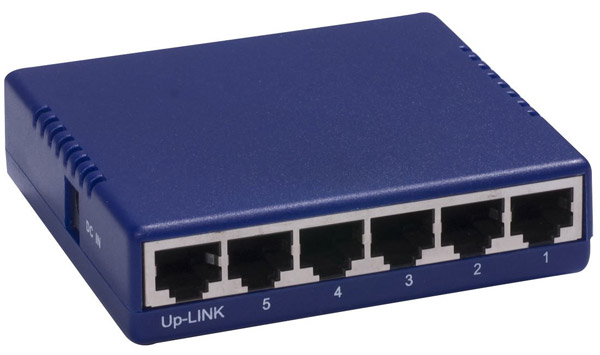
\includegraphics[width=0.8\linewidth]{figures/HUB1}
		\caption{HUB}
		\label{hub1}
	\end{figure}
\end{minipage}
%%%%%%%%%%%%%%%%%%%%%%%%%%%%%%%%%%%%%%%%%%%%%%%%%%%%%%%%%%%%%%%%%%%%%%%%%%%%%%
\begin{minipage}[c]{0.6\textwidth}
	\subsection{Switch}
	An improved version of the Hub that performs the same function as the Hub (links multiple computers or devices together to form a local area network (LAN)), but it's faster and more secure because it sends data in every transmission from sender to receiver and not to all points.
	\subsubsection{Examples}
	\begin{itemize}
		\item TP-Link LS1005G
		\item Cisco Micro switches Series
		\item Linksys LGS328C
		\item MERCUSYS MS105
	\end{itemize}
\end{minipage}%
\hfill
\begin{minipage}[r]{0.40\textwidth}
	
	\begin{figure}[H]
		\centering
		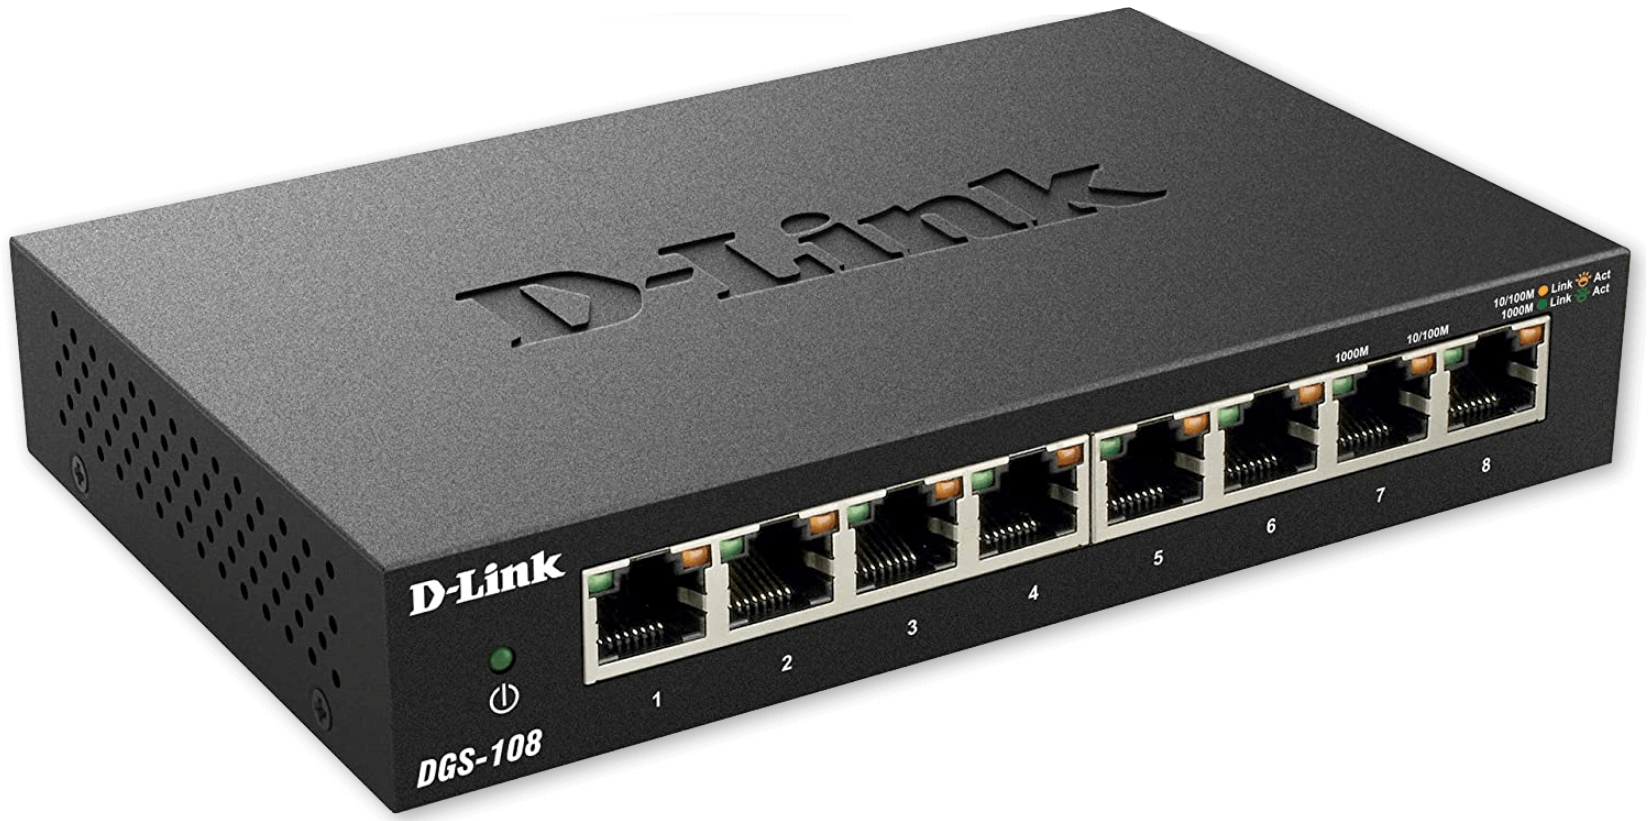
\includegraphics[width=0.8\linewidth]{figures/Switch1}
		\caption{Switch}
		\label{switch1}
	\end{figure}
\end{minipage}
%%%%%%%%%%%%%%%%%%%%%%%%%%%%%%%%%%%%%%%%%%%%%%%%%%%%%%%%%%%%%%%%%%%%%%%%%%%%%%
\begin{minipage}[c]{0.6\textwidth}
	\subsection{Repeater}
	A device that restores the signal and ensures signal integrity in long signal cables. More than one can be placed along the transmission line if the line is long enough.
	\subsubsection{Examples}
	\begin{itemize}
		\item VIMIN 2-Port Outdoor PoE Gigabit Extender
		\item Revotech 2 Port POE Extender
		\item TP-Link RE305 AC1200 Wi-Fi Range Extender
	\end{itemize}
\end{minipage}%
\hfill
\begin{minipage}[r]{0.40\textwidth}
	
	\begin{figure}[H]
		\centering
		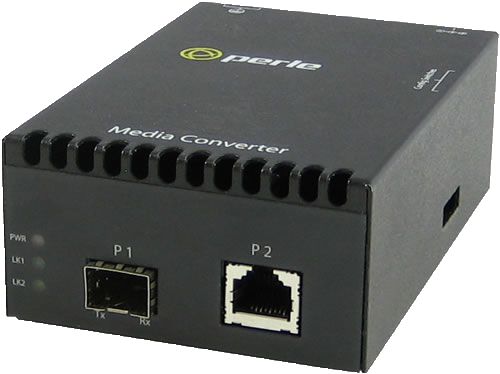
\includegraphics[width=0.8\linewidth]{figures/repeater1}
		\caption{Repeater}
		\label{repeater1}
	\end{figure}
\end{minipage}
%%%%%%%%%%%%%%%%%%%%%%%%%%%%%%%%%%%%%%%%%%%%%%%%%%%%%%%%%%%%%%%%%%%%%%%%%%%%%%
\begin{minipage}[c]{0.6\textwidth}
	\subsection{Access point}
	It can be considered a converter that transforms a wired signal into a wireless one, allowing devices to connect to a wired LAN network via Wi-Fi.
	\subsubsection{Examples}
	\begin{itemize}
		\item Ubiquiti UniFi AC Pro
		\item TP-Link EAP225 Omada
	\end{itemize}
\end{minipage}%
\hfill
\begin{minipage}[r]{0.40\textwidth}
	
	\begin{figure}[H]
		\centering
		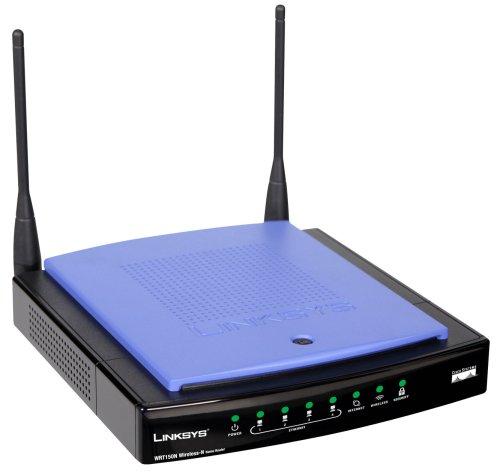
\includegraphics[width=0.8\linewidth]{figures/AP1}
		\caption{Access point}
		\label{AP1}
	\end{figure}
\end{minipage}
%%%%%%%%%%%%%%%%%%%%%%%%%%%%%%%%%%%%%%%%%%%%%%%%%%%%%%%%%%%%%%%%%%%%%%%%%%%%%%
\begin{minipage}[c]{0.6\textwidth}
	\subsection{Router}
	A device that allows communication between networks and enables communication with the network that carries the internet.
	\subsubsection{Examples}
	\begin{itemize}
		\item Cisco RV340 Dual WAN Gigabit Router
		\item ASUS RT-AX88U AX6000 WiFi 6 Router
	\end{itemize}
\end{minipage}%
\hfill
\begin{minipage}[r]{0.40\textwidth}
	
	\begin{figure}[H]
		\centering
		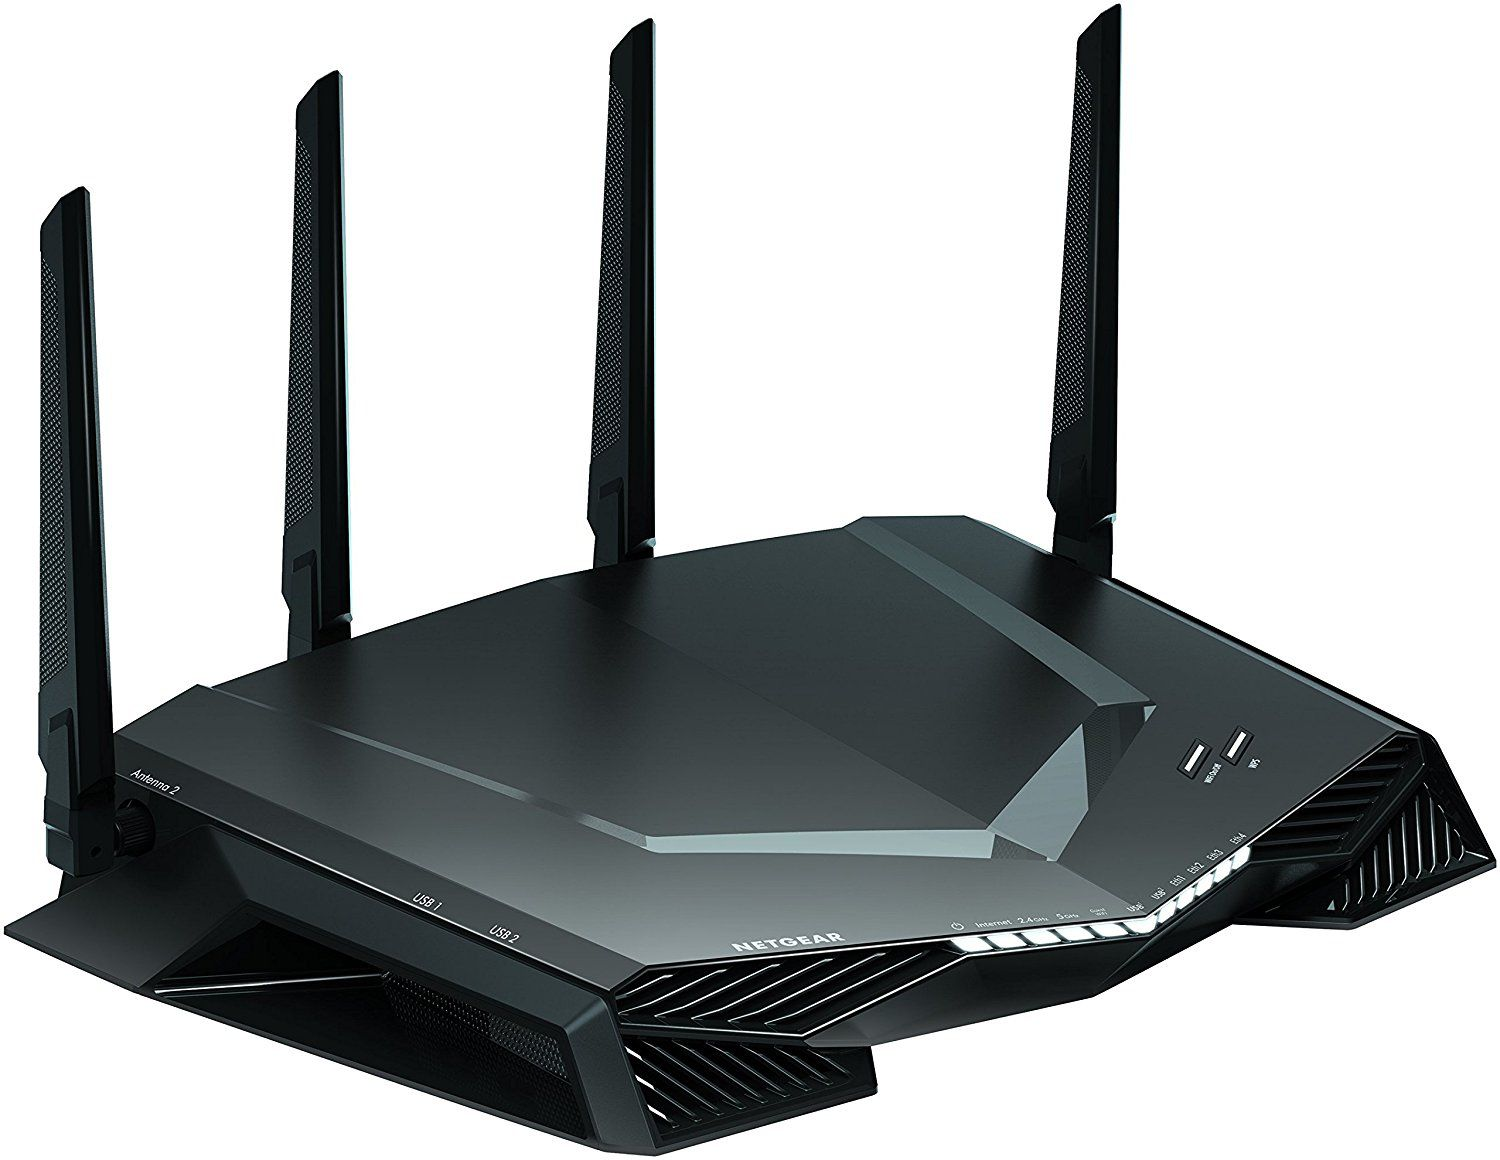
\includegraphics[width=0.8\linewidth]{figures/router1}
		\caption{Router}
		\label{Router}
	\end{figure}
\end{minipage}
%%%%%%%%%%%%%%%%%%%%%%%%%%%%%%%%%%%%%%%%%%%%%%%%%%%%%%%%%%%%%%%%%%%%%%%%%%%%%%
\begin{minipage}[c]{0.6\textwidth}
	\subsection{NIC (Network Interface Card)}
	a hardware that enable the device to directly access the network.
	and there is two types of it:
	\begin{enumerate}
		\item Internal NIC
		plugs into the motherboard directly
		
		\item External NIC
		Wireless and USB based
	\end{enumerate}
	\subsubsection{Examples}
	\begin{itemize}
		\item Intel I350-T2 Gigabit Ethernet NIC
		\item TP-Link TL-WN725N USB Wi-Fi Adapter
	\end{itemize}
\end{minipage}%
\hfill
\begin{minipage}[r]{0.40\textwidth}
	
	\begin{figure}[H]
		\centering
		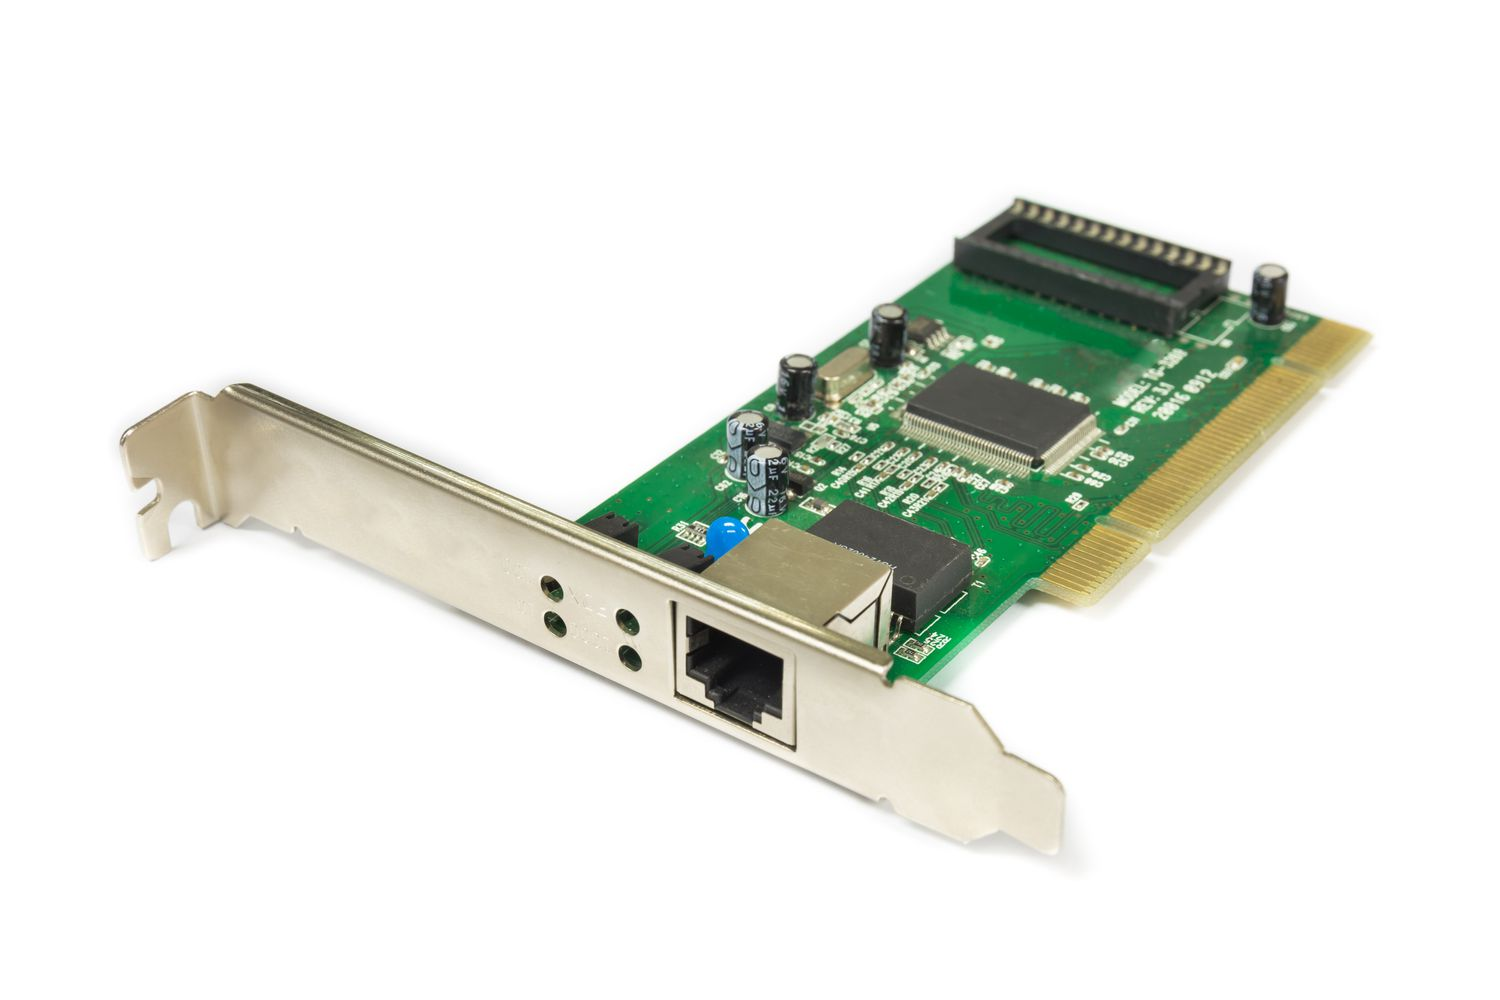
\includegraphics[width=0.45\linewidth]{figures/NIC1}
		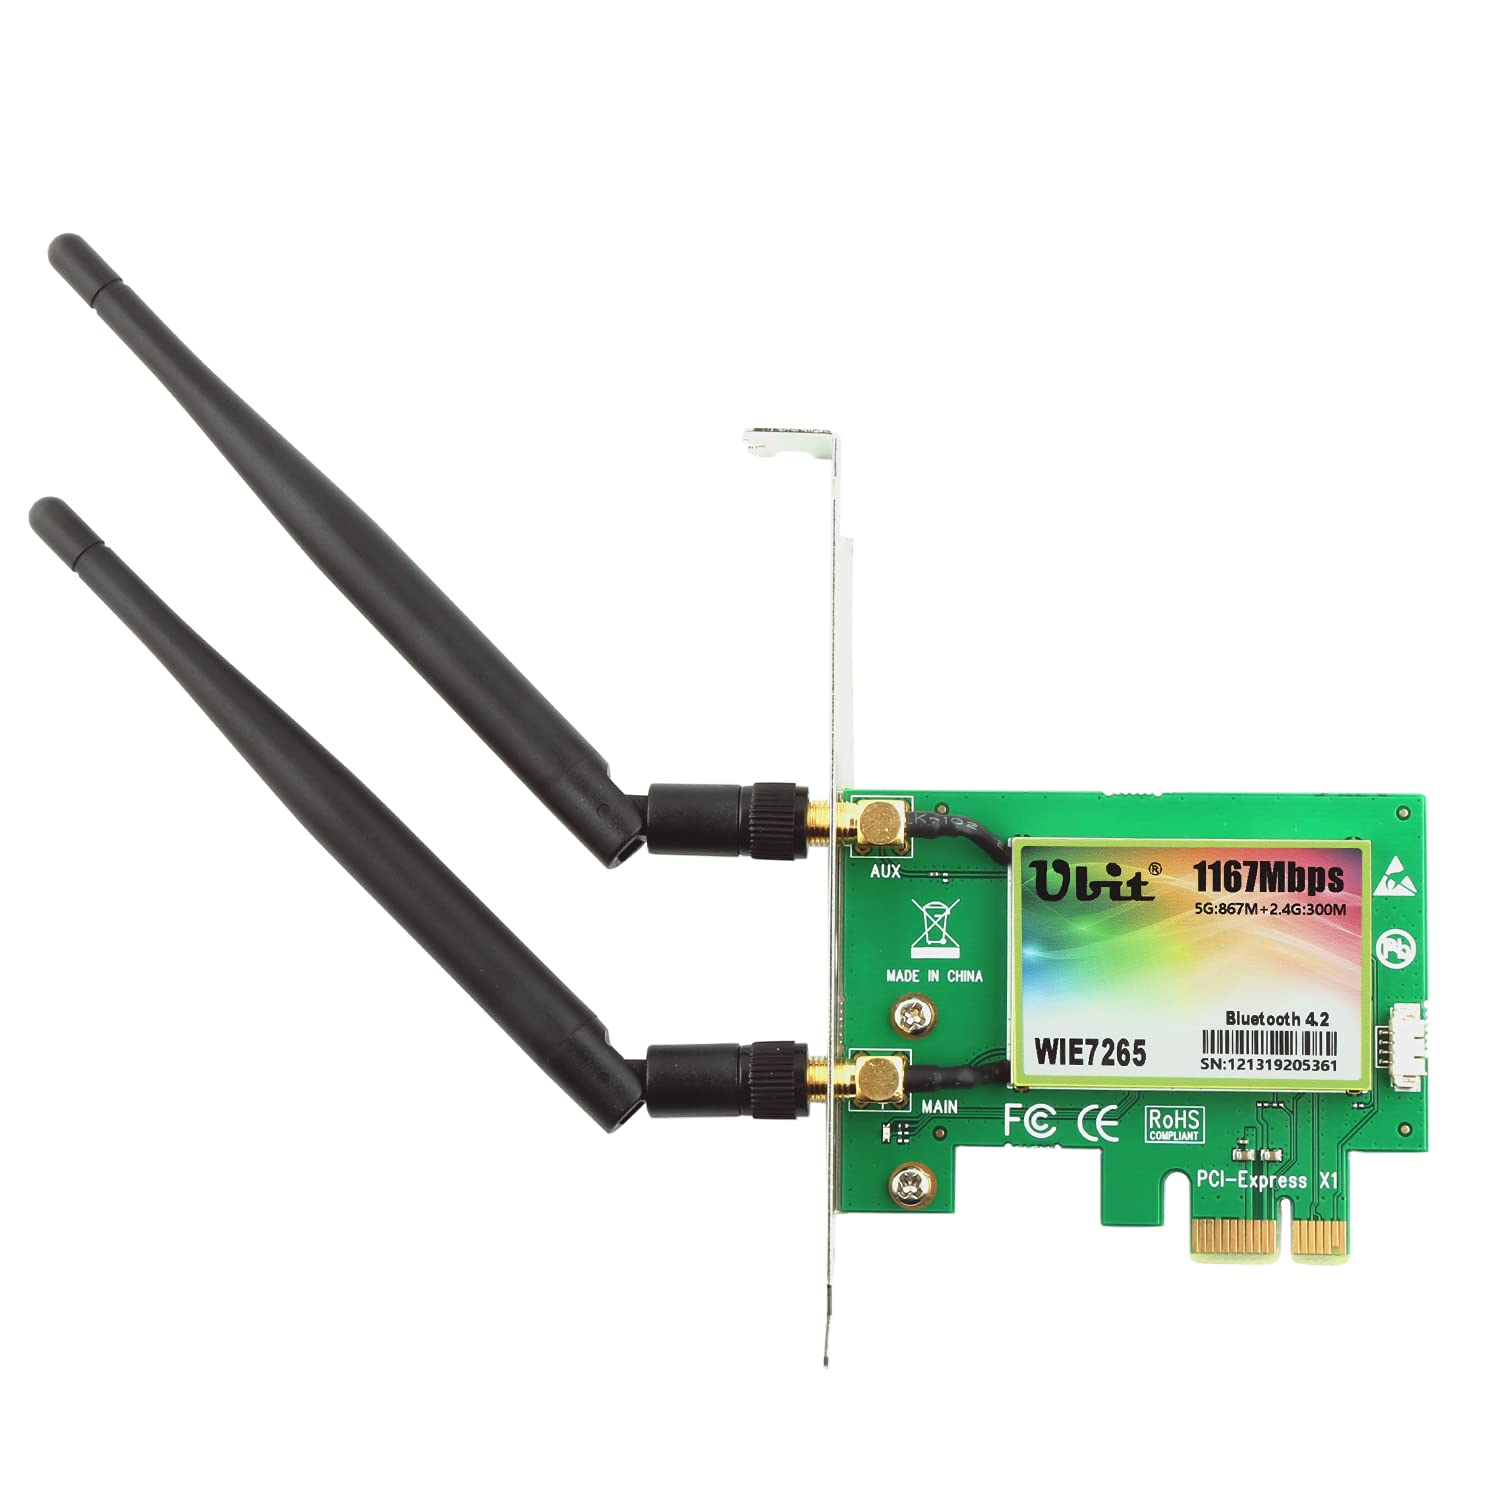
\includegraphics[width=0.45\linewidth]{figures/NIC2}
		\caption{NIC cards}
		\label{NIC}
	\end{figure}
\end{minipage}

%%%%%%%%%%%%%%%%%%%%%%%%%%%%%%%%%%%%%%%%%%%%%%%%%%%%%%%%%%%%%%%%%%%%%%%%%%%%%%
\begin{minipage}[c]{0.6\textwidth}
	\subsection{Mac address}
	A physical and globally unique hardware identifier assigned to a Network Interface Card (NIC) at the manufacturing stage. It operates at the Data Link Layer (Layer 2) of the OSI model and consists of a 48-bit (6-byte) hexadecimal address used to facilitate local frame delivery within the same network segment.
\end{minipage}%
\hfill
\begin{minipage}[r]{0.40\textwidth}
	
	\begin{figure}[H]
		\centering
		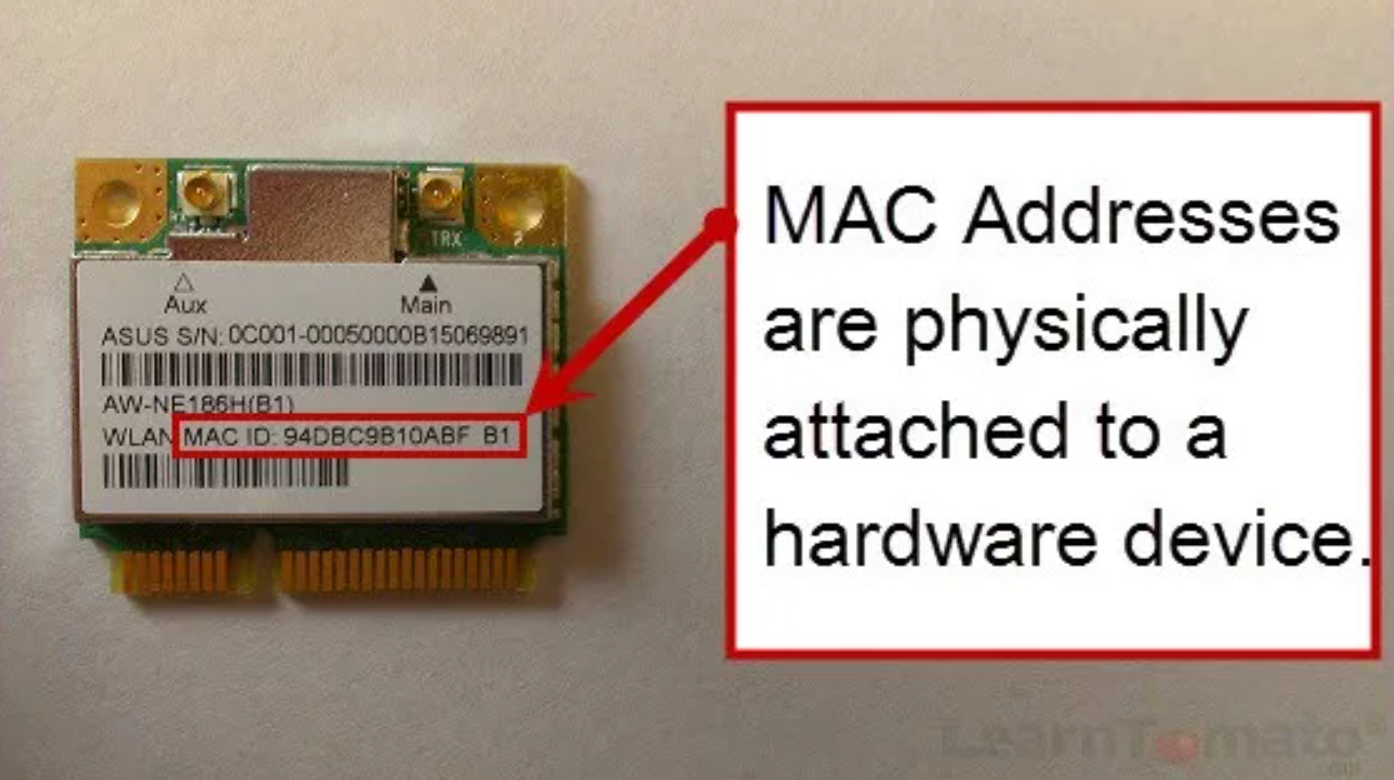
\includegraphics[width=0.8\linewidth]{figures/MAC1}
		\caption{Mac address}
		\label{MAC}
	\end{figure}
\end{minipage}

\hfill
\begin{minipage}[c]{0.6\textwidth}
	\subsection{IP address}
	A logical layer 3 network address assigned to identify devices and route traffic across interconnected networks. It exists in two main formats: IPv4 (32-bit address space, e.g., 192.168.1.1) and IPv6 (128-bit address space to prevent IP exhaustion). It is divided into Network ID and Host ID portions, allowing packets to be properly routed across public and private subnets.
\end{minipage}%
\hfill
\begin{minipage}[r]{0.40\textwidth}
	
	\begin{figure}[H]
		\centering
		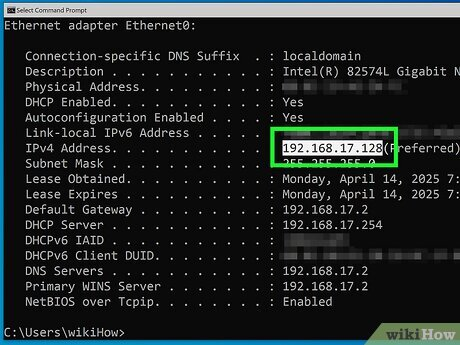
\includegraphics[width=0.7\linewidth]{figures/IP1}
		\caption{IP address}
		\label{fig:ip1}
	\end{figure}
\end{minipage}



\newpage

\subsection{Protocols}
A standardized set of rules and conventions that govern data formatting, transmission, and error handling between network entities across different layers:
\begin{itemize}
	\item \textbf{HTTP/HTTPS:} Web browsing protocols (HTTPS adds SSL/TLS encryption for secure data transfer).
	\item \textbf{FTP:} File Transfer Protocol used for uploading and downloading files over a client-server architecture.
	\item \textbf{RDP:} Remote Desktop Protocol allowing users to visually control a computer remotely over a network connection.
\end{itemize}
\begin{figure}[!h]
	\centering
	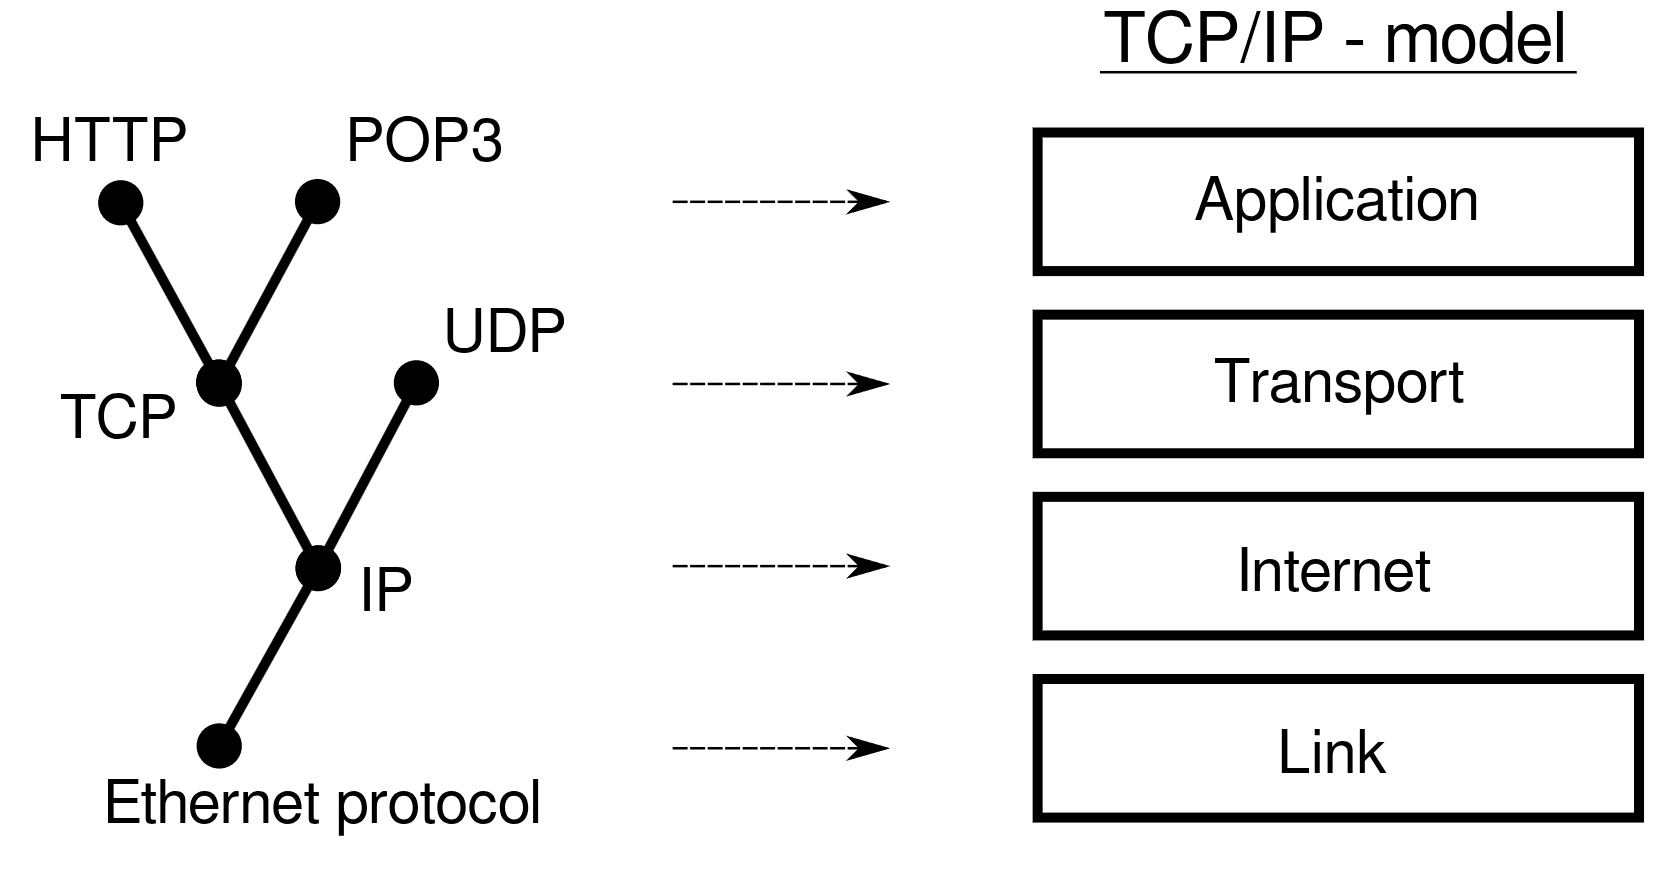
\includegraphics[width=0.7\linewidth]{figures/protocols1}
	\caption{TCP/IP model}
	\label{fig:protocols1}
\end{figure}

\noindent\rule{\textwidth}{0.4pt}
\section{Network Classifications}
\begin{figure}[H]
	\centering
	\begin{tikzpicture}[
		node distance = 1.2cm and 0.6cm,
		% نمط العنوان الرئيسي في المنتصف
		titlebox/.style = {
			draw=black,
			fill=black,
			text=white,
			font=\bfseries\Large,
			align=center,
			rounded corners=8pt,
			inner sep=12pt,
			minimum width=8cm,
			drop shadow
		},
		% نمط الصناديق الفرعية الثلاثة
		itembox/.style = {
			draw=black,
			fill=white,
			thick,
			rounded corners=6pt,
			align=center,
			inner sep=10pt,
			minimum width=4.5cm,
			minimum height=2cm,
			font=\small
		},
		% نمط الأسهم الموجهة
		arrowstyle/.style = {
			-Stealth,
			thick,
			color=black,
			line width=1.5pt
		}
		]
		
		% 1. العنوان الرئيسي في المنتصف فوق
		\node (title) [titlebox] {Network Classifications};
		
		% 2. العناصر الثلاثة تحت العنوان (العنصر الأوسط تحت العنوان مباشرة، والآخران على جانبيه)
		\node (item2) [itembox, below=of title] {
			\textbf{\color{black} According to network topology}\\[0.5em]
			\textit{How the computers are connected?}
		};
		
		\node (item1) [itembox, left=of item2] {
			\textbf{\color{black} According to Covered Area}\\[0.5em]
			\textit{How large is the network?}
		};
		
		\node (item3) [itembox, right=of item2] {
			\textbf{\color{black} According to network model}\\[0.5em]
			\textit{What type of model?}
		};
		
		% 3. رسم الأسهم المنحنية (Curved Arrows)
		\draw [arrowstyle] (title.south west) to[out=210, in=90] (item1.north);
		\draw [arrowstyle] (title.south) -- (item2.north);
		\draw [arrowstyle] (title.south east) to[out=330, in=90] (item3.north);
		
	\end{tikzpicture}
\end{figure}

\subsection{According to Covered Area}


\begin{minipage}[c]{0.6\textwidth}
	\subsubsection{Personal Area Networks (PAN)}
	a computer network for interconnecting
	devices centered on an individual person's
	workspace.
	
	provides data transmission among
	devices such as computers, smartphones,
	tablets and personal digital assistants
	\subsubsection{Examples}
	\begin{itemize}
		\item Connecting a smartphone to a smartwatch via Bluetooth.
		\item Connecting wireless Bluetooth earbuds to a laptop.
		\item Transferring files between two phones using Wi-Fi Direct or AirDrop.
		\item Connecting a wireless mouse or keyboard to a computer using a USB dongle.
	\end{itemize}
\end{minipage}%
\hfill
\begin{minipage}[r]{0.40\textwidth}
	
	\begin{figure}[H]
		\centering
		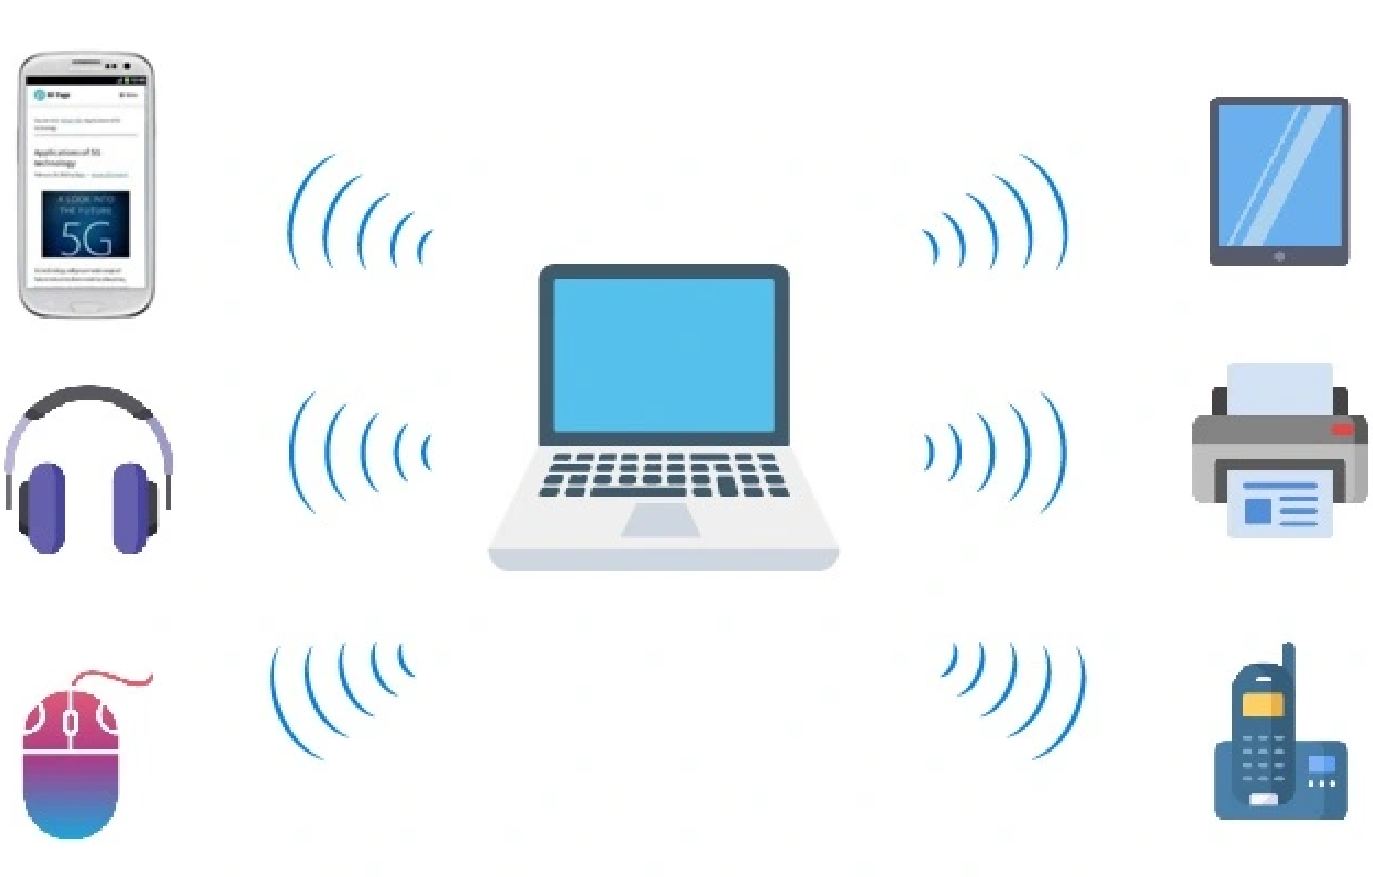
\includegraphics[width=0.7\linewidth]{figures/PAN}
		\caption{PAN Network}
		\label{PAN}
	\end{figure}
\end{minipage}

\begin{minipage}[c]{0.6\textwidth}
	\subsubsection{Local Area Networks (LAN)}
	a computer network that interconnects computers within a limited area such as a residence, school, laboratory, university campus or office building.
	
	provides high data transfer rates, low latency, and secure communication among connected devices like PCs, servers, and network printers.
	\subsubsection{Examples}
	\begin{itemize}
		\item A home Wi-Fi network connecting PCs, smart TVs, and phones.
		\item An office network connecting workstations to a central server and shared printer.
		\item A computer lab in a school linked via Ethernet switches.
		\item Interconnected devices in a university building sharing local resources.
	\end{itemize}
\end{minipage}%
\hfill 
\begin{minipage}[r]{0.40\textwidth}
	
	\begin{figure}[H]
		\centering
		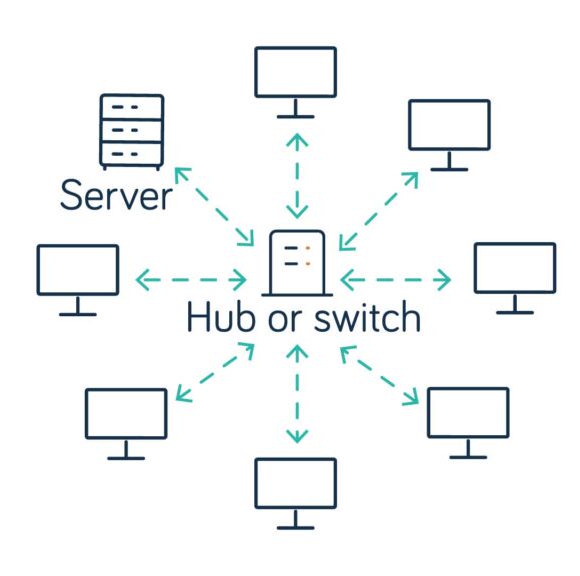
\includegraphics[width=0.7\linewidth]{figures/LAN}
		\caption{LAN Network}
		\label{LAN}
	\end{figure}
\end{minipage}

\begin{minipage}[c]{0.6\textwidth}
	\subsubsection{Metropolitan Area Networks (MAN)}
	a computer network that covers a larger geographic area than a LAN, spanning an entire city or a large town.
	
	provides high-speed connectivity to bridge multiple LANs across a town or city, typically managed by a single entity or service provider.
	\subsubsection{Examples}
	\begin{itemize}
		\item A city-wide cable television network delivering broadband internet.
		\item A municipal network connecting various government offices across a city.
		\item A university campus network connecting separate branch buildings across town.
		\item A local bank branch network connected to a city headquarters.
	\end{itemize}
\end{minipage}%
\hfill 
\begin{minipage}[r]{0.40\textwidth}
	
	\begin{figure}[H]
		\centering
		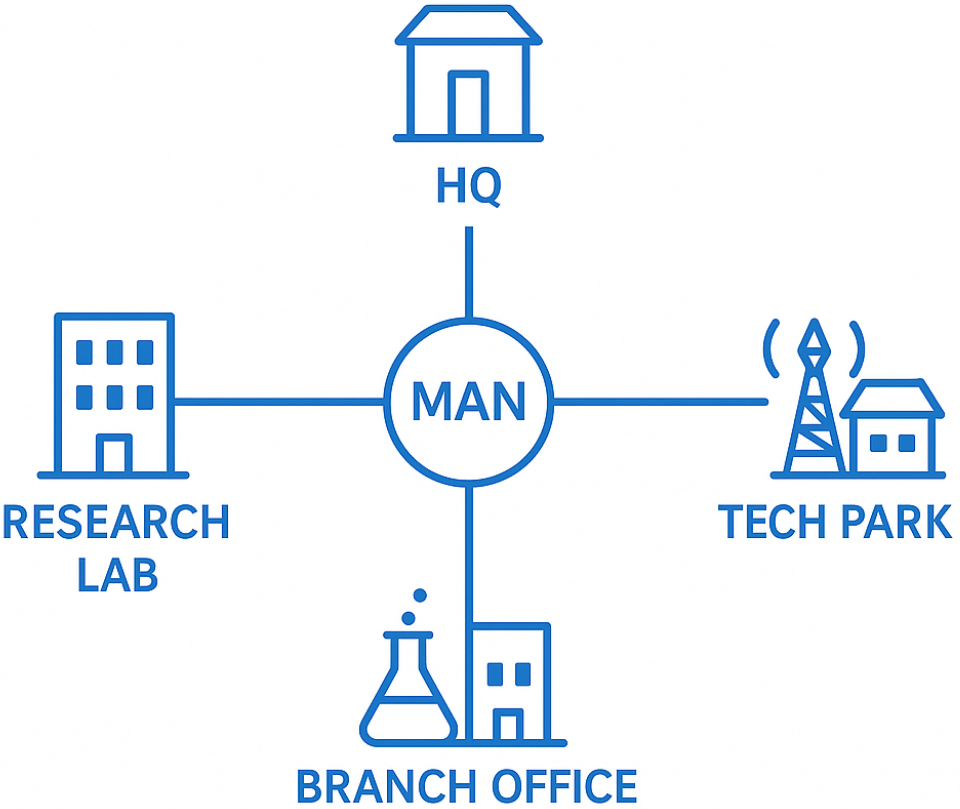
\includegraphics[width=0.7\linewidth]{figures/MAN}
		\caption{MAN Network}
		\label{MAN}
	\end{figure}
\end{minipage}

\begin{minipage}[c]{0.6\textwidth}
	\subsubsection{Wide Area Networks (WAN)}
	a telecommunications network that extends over a large geographic distance, often crossing cities, countries, or continents.
	
	provides long-distance data transmission, connecting multiple smaller networks (LANs and MANs) together using public or private transport systems.
	\subsubsection{Examples}
	\begin{itemize}
		\item The global Internet connecting millions of devices worldwide.
		\item A multinational corporation linking offices in different countries via VPN.
		\item ATM networks of a national bank connected across multiple regions.
		\item Cloud infrastructure interconnecting international data centers.
	\end{itemize}
\end{minipage}%
\hfill
\begin{minipage}[r]{0.40\textwidth}
	
	\begin{figure}[H]
		\centering
		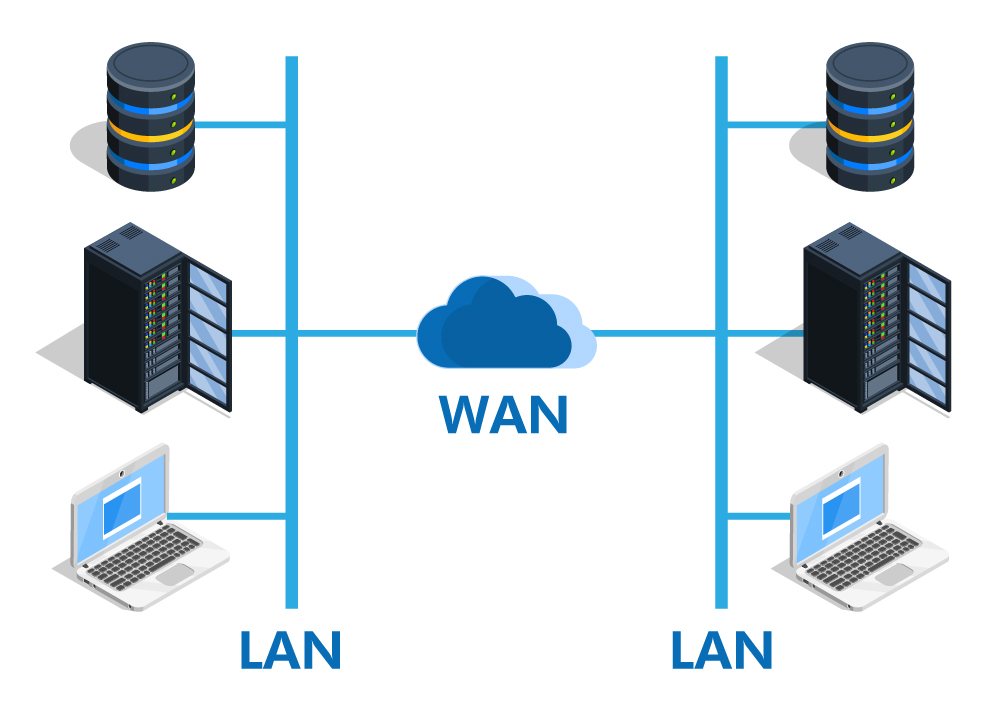
\includegraphics[width=0.7\linewidth]{figures/WAN}
		\caption{WAN Network}
		\label{WAN}
	\end{figure}
\end{minipage}





